\documentclass[12pt]{article}

\usepackage{fullpage}
\usepackage{graphicx, rotating, booktabs} 
\usepackage{times} 
\usepackage{natbib} 
\usepackage{indentfirst} 
\usepackage{setspace}
\usepackage{grffile} 
\usepackage{hyperref}
\usepackage{adjustbox}
\setcitestyle{aysep{}}


\singlespace
\title{
\textbf{Appendix: Reassessing the Public Goods Theory of Alliances}
	}
%\author{Joshua Alley\footnote{Graduate Student,
%Department of Political Science, Texas A\&M University.}}

\bibliographystyle{apsr}

\begin{document}

\maketitle 

\doublespace

This appendix contains supporting materials for the test of Hypothesis 1 in ``Reassessing the Public Goods Theory of Alliances.'' 
Section 1 provides more detail about the variables in the model and Section 2 shows that results from the hierarchical model are accurate. 


\section{Variables} 


Olson and Zeckhauser use GDP to measure state size, so I constructed a measure of GDP using data from the Maddison Project, which provides longer historical coverage \citep{Boltetal2018}. 
I then take the natural log of GDP to address the variable's skewed distribution. 
I use military spending data from the Correlates of War Project \citep{SingerCINC1988}.  
All alliance membership data comes from Version 4 of the Alliance Treaty Obligations and Provisions (ATOP) data \citep{Leedsetal2002}.  


My dependent variable is percentage changes in military spending. 
Olson and Zeckhauser use defense spending as a share of GDP as their dependent variable, which is the source of previously described identification problems \citep{Kronmal1993, PluemperNeumayer2015}. 
I use percentage changes instead of the defense burden because this measure gives a sense of burdens from changing defense budgets with a lower risk of spurious inferences. 
Annual percentage changes in spending is the change in military spending as a share of the previous year's budget:


\begin{equation}
\mbox{\% Change Military Spending} = \frac{\mbox{Mil. Ex.}_t - \mbox{Mil. Ex.}_{t-1} }{ \mbox{Mil. Ex.}_{t-1} } = \frac{\Delta \mbox{Mil. Ex.} }{ \mbox{Mil. Ex.}_{t-1} }
\end{equation} 


Measuring percentage changes in spending matches Olson and Zeckhauser's emphasis on how alliance participants allocate resources to the military.
Positive percentage changes in spending imply an expanding defense budget and higher defense burden, all else equal.
Moreover, using percentage changes in spending mitigates the risk of spurious inferences due to non-stationarity in panel data. 
The log-level of military spending is not mean-reverting in long panels.
A differenced military spending variable has increasing variance over time, as budgets expand and generate larger changes. 
Modeling the DV in levels or changes might lead to spurious inferences \citep{GrangerNewbold1974}. 


Using percentage changes in military spending as the dependent variable benchmarks changes to budget size. 
This facilitates comparisons across states and years. 
A 2\% change is an equally burdensome increase in the defense budget for large and small states, all else equal. 


Besides the economic weight values in \textbf{Z}, I controlled for other variables that are correlated with alliance participation and military spending. 
I adjusted for international war \citep{Reiteretal2016}, civil war participation \citep{SarkeesWayman2010}, and a count of annual MIDs \citep{Gibleretal2016}. 
I also included measures of regime type, external threat \citep{LeedsSavun2007}, GDP, and the Cold War era. 

 


\section{Multilevel Model}

This section describes the priors on the multilevel model, convergence diagnostics for the Hamiltonian Monte Carlo, and results from running the same model on a sample of states with at least one alliance. 


\subsection{Priors} 

All priors are specified to be weakly informative relative to the scale of the data \citep{Gelmanetal2017}. 
I summarize the prior distributions for each set of parameters in \autoref{tab:priors}. 
$p(\nu)$ is a well-behaved prior for the degrees of freedom in a t-distribution \citep{JuarezSteele2010}. 
Given that the median percentage change in military expenditures is 0.06, the priors are quite diffuse. 


\begin{table} % Create a table of priors.
\begin{center}
\begin{tabular}{c} 
$ p(\alpha) \sim N(0, 1)$  \\
$ p(\sigma) \sim \mbox{half-}N(0, 1) $ \\
$ p(\alpha^{yr}) \sim N(0, \sigma^{yr}) $ \\ 
$ p(\sigma^{yr}) \sim N(0, 1) $ \\
$ p(\alpha^{st}) \sim N(0, \sigma^{st}) $ \\ 
$ p(\sigma^{st}) \sim \mbox{half-}N(0, 1) $ \\ 
$ p(\gamma) \sim N(\theta, \sigma^{all}) $ \\ 
$ p(\theta) \sim N(0, .5) $ \\
$ p(\sigma^{all}) \sim \mbox{half-}N(0, 1) $ \\
$ p(\beta) \sim N(0, 1) $ \\
$ p(\nu) \sim gamma(2, 0.1)$ 
\end{tabular} 
\caption{Summary of Priors in Multilevel Model} 
\label{tab:priors}
\end{center} 
\end{table} 


To facilitate estimation, I use a non-centered parameterization for the state and year varying intercepts, as well as the $\gamma$ parameters \citep{BetancourtGirolani2015}. 
A non-centered parameterization decouples the mean and variance to express an equivalent prior, which makes sampling easier. 
I also employ a sparse matrix representation of the alliance membership matrix $\textbf{Z}$ to speed up estimation. 


\subsection{Convergence} 


There were no divergent iterations in sampling. 
However, there are other threats to inference from the posterior samples. 
Given heavy tails in percentage changes of military spending, STAN might have struggled to explore the posterior distribution. 


Energy plots can diagnose this problem. 
\autoref{fig:energy-plot} plots the marginal energy distribution and the first differenced distribution. 
If the two histograms do not overlap, sampling was impeded by heavy tails. 
The substantial overlap in the distributions for all four chains in \autoref{fig:energy-plot} indicates this was not a problem. 


\begin{figure}
	\centering
		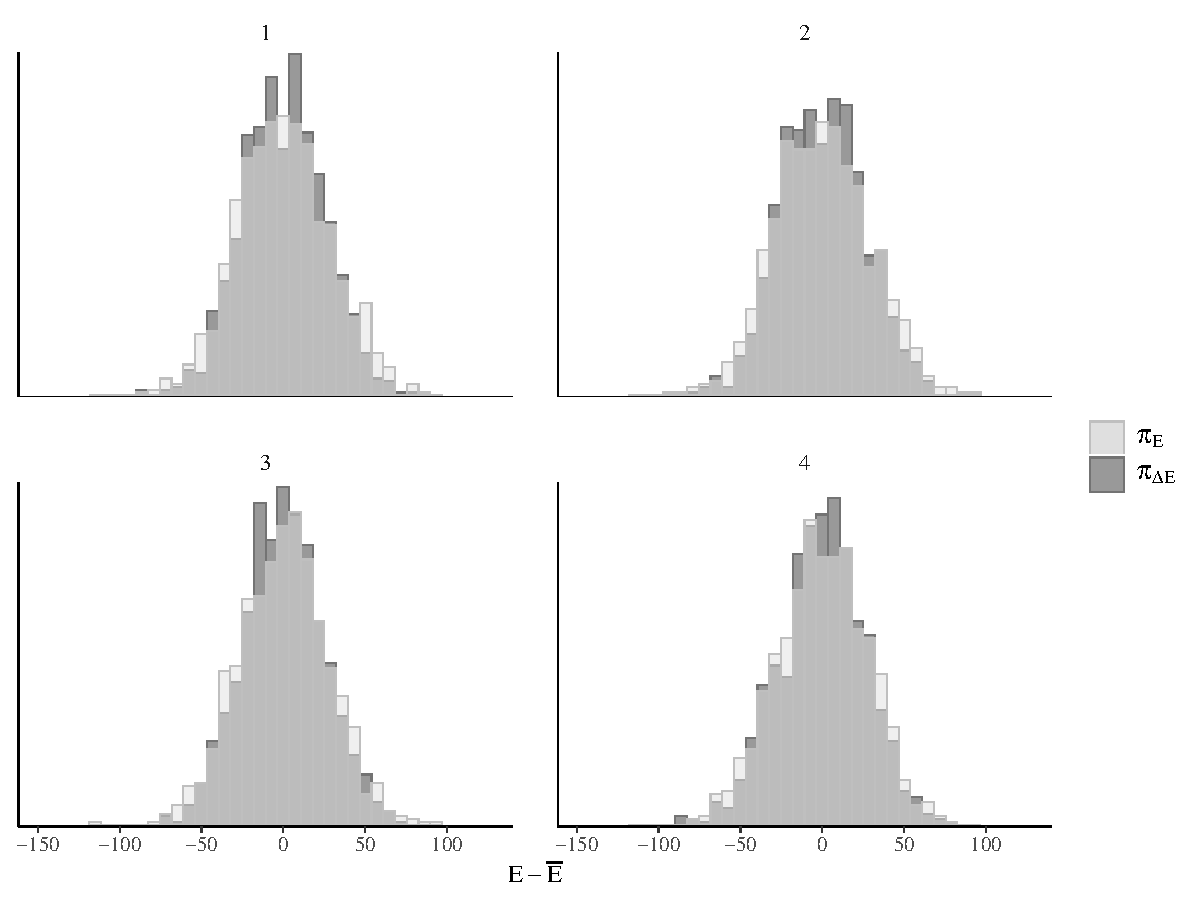
\includegraphics[width=0.55\textwidth]{energy-plot.pdf}
	\caption{Energy plot of multilevel model results. Greater overlap in the two histograms indicates adequate exploration of the posterior distribution. }
	\label{fig:energy-plot}
\end{figure}


The split $\hat{R}$ statistic is another way to assess convergence. 
$\hat{R}$ compares the behavior of each chain by measuring the ratio of the average variance of draws within each chain to the variance of the pooled draws across chains. 
When $\hat{R}$ is close to 1, all the chains have similar variance, and are therefore in equilibrium. 


The standard heuristic is that an $\hat{R}$ greater than 1.1 is problematic. 
\autoref{fig:rhat-plot} plots the $\hat{R}$ statistic for every parameter in the model. 
No parameters generate concern, even at a more conservative threshold of 1.05. 


\begin{figure}[htbp]
	\centering
		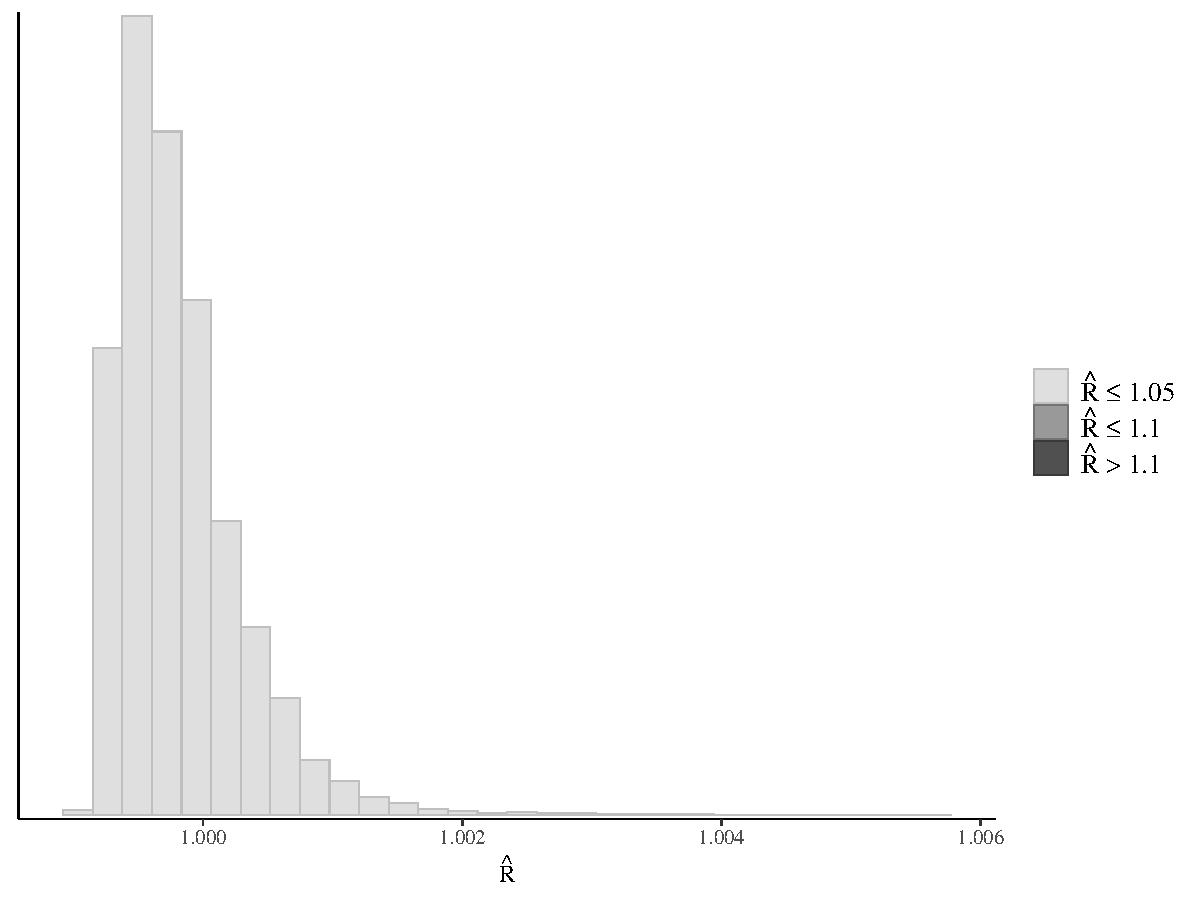
\includegraphics[width=0.55\textwidth]{rhat-plot.pdf}
	\caption{Histogram of split $\hat{R}$ statistic for all parameters in the multilevel model.}
	\label{fig:rhat-plot}
\end{figure}


\subsubsection{Inferences from Simulated Data}


To assess if the model gives reasonable answers, I simulated data and associated parameters, then re-estimated the model on the simulated data.
The model is a good fit if the credible intervals contain the known parameter values for the simulated data. 
This process checks whether the model can recover parameters from a known data-generating process that matches the model. 


I simulate a hypothetical dataset with 5000 observations of 50 states observed over 200 years. 
There are 200 alliances in this data, and 2 state-level control variables. 
The hypothetical outcome is drawn from a Cauchy distribution with mean 0 and a scale of .25, which is more heavy-tailed than even my observed data. 


I then simulate 2,000 draws of the outcome using the generated quantities block in STAN. 
The next step is selecting one of those draws of the outcome--- which includes the value of the outcome for each observation and the associated parameter values. 
I select the 12th draw from the posterior and check whether after estimating the model on these data, the credible intervals include zero. 


I focus on inferences about the $\gamma$, $\theta$ and $\sigma_{all}$ parameters, because these are essential to testing the public goods argument. 
As \autoref{fig:theta-sim-res} and \autoref{fig:sall-sim-res} show, the posteriors accurately capture the known values of the hyper-parameters $\theta$ and $\sigma_{all}$. 
In these figures, the true parameter value is marked with a thick black line, while the light gray shaded area shows the 90\% credible interval. 


\begin{figure}[htbp]
	\centering
		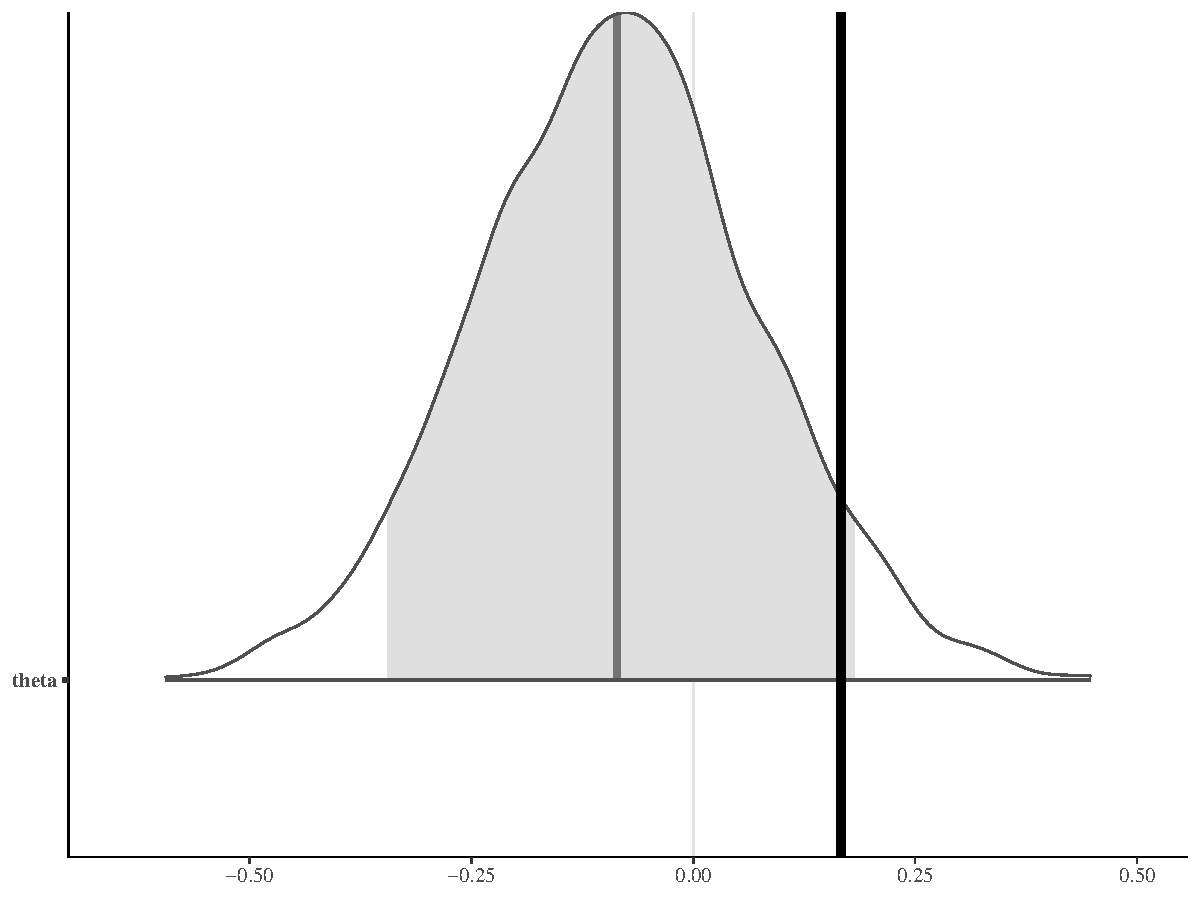
\includegraphics[width=0.65\textwidth]{theta-sim-res.pdf}
	\caption{Posterior estimates and known parameter value for the alliance hyperparameter $\theta$. The dark gray bar marks the posterior mean, while the shaded area captures the 90\% credible interval. The black line marks the known, ``true'' $\theta$ value, which falls within the 90\% interval.}
	\label{fig:theta-sim-res}
\end{figure}


\begin{figure}[htbp]
	\centering
		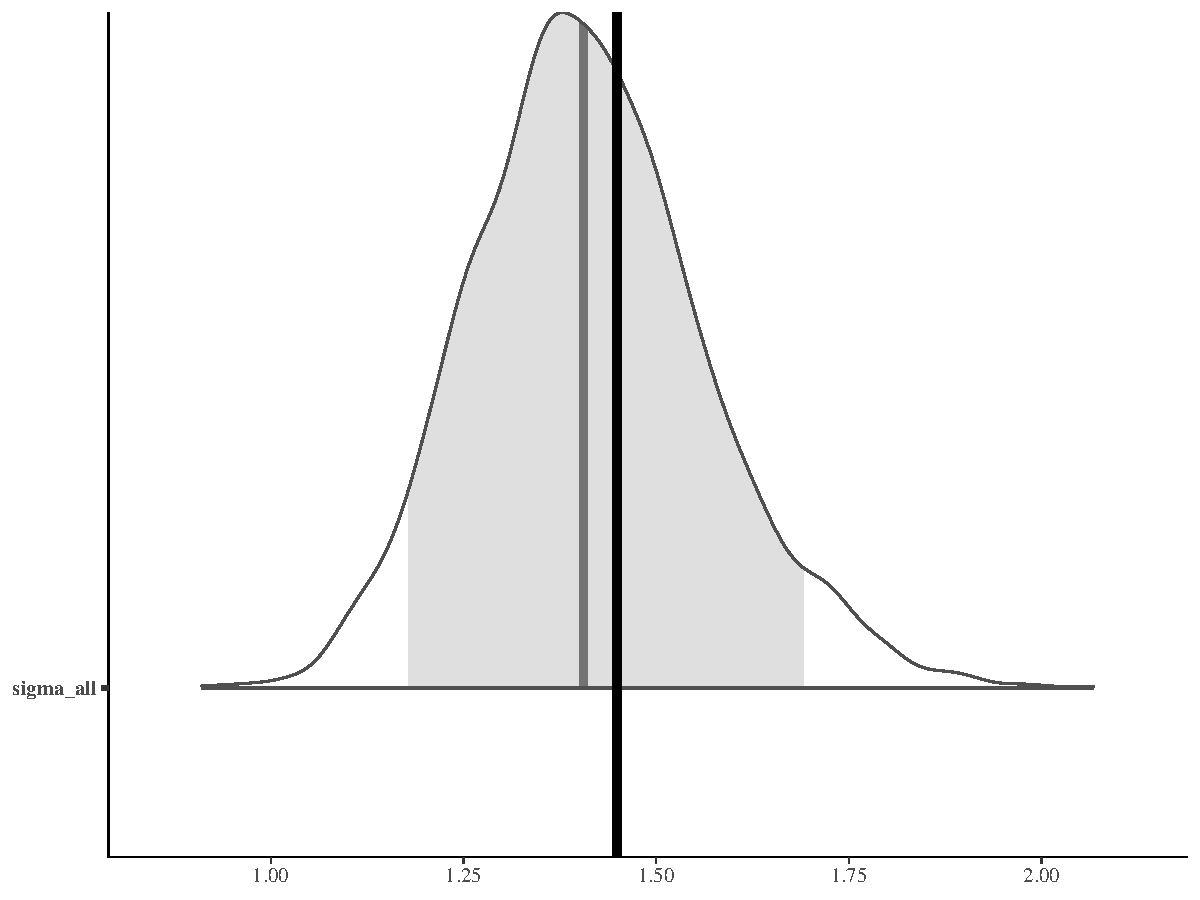
\includegraphics[width=0.65\textwidth]{sall-sim-res.pdf}
	\caption{Posterior estimates and known parameter value for the alliance hyperparameter $\sigma_{all}$. The dark gray bar marks the posterior mean, while the shaded area captures the 90\% credible interval. The black line marks the known, ``true'' $\sigma_{all}$ value, which falls within the 90\% interval.}
	\label{fig:sall-sim-res}
\end{figure}


Because graphical presentation of the 200 $\gamma$ parameters is more difficult, I calculated whether the credible interval contained the known parameter. 
184 of the 200 intervals include the ``true'' $\gamma$ value, which is a 92\% success rate. 
Given the number of parameters and potential simulation variance, such accuracy is tolerable. 
Simulating data and recovering known parameters shows that the model estimates are reasonable approximations of the data-generating process. 
 



\subsection{Alternative Sample} 


It is possible that estimating a model on the full sample of states makes misleading comparisons by including states with no alliances.
This adds many zeros to the membership matrix \textbf{Z}. 
To check whether inferences are sensitive to including states with no alliance participation, I re-fit the multilevel model on a sample of only states with at least one alliance. 
This reduced the sample size from 9,961 observations to 5,222, but the results are relatively unchanged. 


All 285 treaties have a negative mean $\gamma$ estimate, and none have a 90\% credible interval that excludes zero.
The overall mean $\theta$ is more negative in this sample and the $\gamma$ estimates remain tightly clustered around that mean. 
Thus as \autoref{fig:sample-comp-gamma} shows, the distribution of the association between treaty contribution and spending across alliances is more negative in the alliance members sample. 
This figure overlays the distribution of the mean $\gamma$ parameters in each sample. 


\begin{figure}
	\centering
		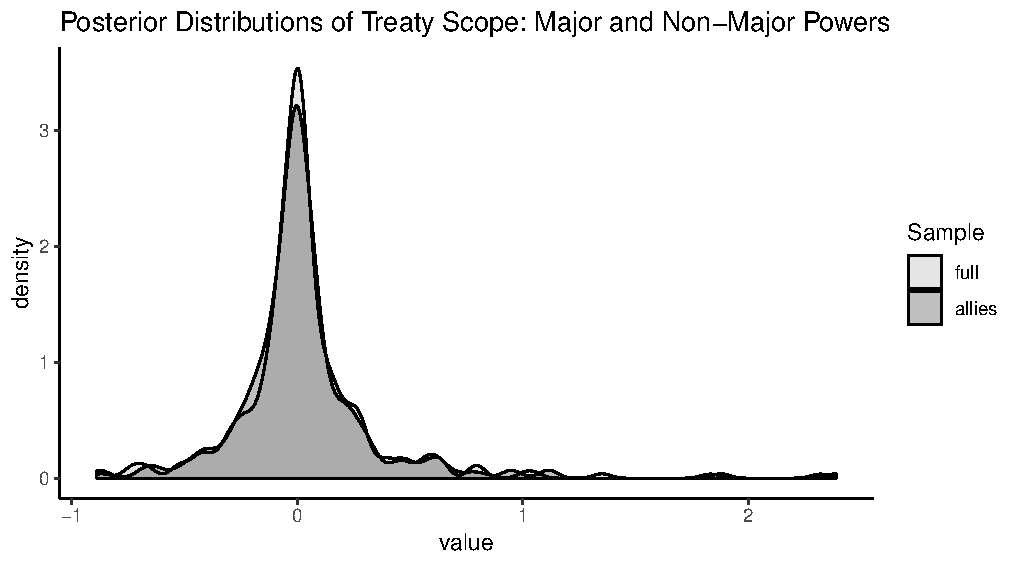
\includegraphics[width=0.95\textwidth]{sample-comp-gamma.pdf}
	\caption{Comparison of the distribution of posterior mean $\gamma$ parameters in full sample and a sample of only alliance participants. The darker gray distribution is the mean of the $\gamma$ parameters in the sample of alliance members. The impact of treaty contribution on percentage changes in military spending is more negative in the alliance-members only sample.}
	\label{fig:sample-comp-gamma}
\end{figure}


Therefore, inferences about the impact of treaty contribution on percentage changes in military spending are unchanged if the sample is restricted only to alliance members. 
Increasing a state's share of total allied GDP leads to a more negative effect on treaty spending in expectation. 
I am still unable to identify any reliably positive $\gamma$ parameters, which contradicts the free-riding hypothesis. 







\newpage
\singlespace


\bibliography{../../../MasterBibliography} 





\end{document}
